\documentclass[12pt,english]{article}
\usepackage[utf8]{inputenc}
\usepackage{tgpagella} % Palatino text only
\usepackage{mathpazo}  % Palatino math & text
\usepackage[left=1.5in,right=1.5in,top=1.5in,bottom=1.5in]{geometry}
% \linespread{1.5}
% \usepackage[super,comma,sort]{natbib}
\usepackage[round,sort&compress]{natbib}
\usepackage{url} % [hyphens]
\usepackage[hyperpageref]{backref} % back references biblio. Needs latexmk at compilation.
\usepackage[pagebackref]{hyperref}
% \usepackage{multibib} % incompatible with backref
\hypersetup{
  colorlinks=true, % breaklinks=true,
  urlcolor=purple,    % color of external links
  linkcolor=blue,  % color of toc, list of figs etc.
  citecolor=violet,   % color of links to bibliography
}
\usepackage{bm}
\usepackage{indentfirst}
\usepackage{tocbibind}
\setcitestyle{aysep={}} 
\usepackage{amsmath}
\usepackage{amssymb}
\usepackage{eurosym}
\usepackage{amsfonts}
\usepackage{enumerate}
\usepackage{babel}
\usepackage{caption}
\usepackage{supertabular}
\usepackage{tabularx}
\usepackage{float}
\usepackage{dsfont}
\usepackage{fancyvrb}
\usepackage{verbatim}
\usepackage{enumitem}
\usepackage{setspace}
\usepackage{comment}
\usepackage{subcaption}
\usepackage{graphicx}
\usepackage{tikz}
\usepackage{gensymb}
\usepackage{textcomp}

\usepackage{tabulary}
\usepackage{tabularx}
\usepackage{booktabs}
\usepackage{fullpage}
\usepackage{morefloats}
\usepackage{makecell}
\usepackage{lscape}
\usepackage{pdflscape}
\usepackage{longtable}
\usepackage{rotating}
\usepackage{fancyhdr}
\usepackage{tocloft}
\usepackage{titletoc}
\usepackage[export]{adjustbox}
\usepackage[anythingbreaks]{breakurl} % for links
\usepackage{multicol}
\newsavebox\ltmcbox % For net gain table over two columns
%\usepackage[nomarkers,figuresonly]{endfloat} % Figures at the end
%\usepackage[section,below]{placeins} % Floats placed in the section they appear in.
\renewcommand{\floatpagefraction}{.9}

\title{A Global Wealth Tax -- Policy Brief
} 

\author{Adrien Fabre\footnote{CNRS, CIRED. E-mail: fabre.adri1@gmail.com (corresponding author).}} 

\date{\today} 

\begin{document}

\maketitle

\begin{center}
{\textbf{\href{https://github.com/bixiou/global_tax_attitudes/raw/main/paper/policy_brief_tax.pdf}{Link to most recent version}}}
\end{center}

\begin{figure}[h!]
  \caption{Support for a Global Wealth Tax (in percent).}\label{fig:support}
  \makebox[\textwidth][c]{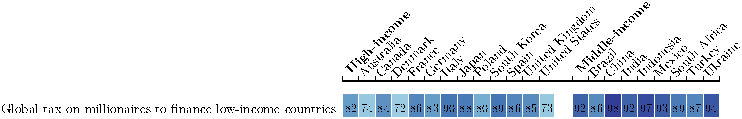
\includegraphics[width=1.2\textwidth]{../figures/OECD/Heatplot_global_tax_attitudes_tax_share.pdf}} 
\end{figure}

\section{Introduction}\label{sec:intro}

\citet{fabre_international_2023} survey attitudes toward global policies in 20 among the largest countries and find near consensus for a global tax on millionaires that would finance low-income countries. The world's richest 1\% (those with a wealth above \euro{}900,000) own 38\% of global wealth \citep{chancel_world_2022}, and the wealth in excess of \euro{}1 million represents 24\% of global wealth. It is logical that the other 99\% massively support taxing the wealthiest. What is more interesting, 90\% of Americans and 92\% of Europeans want to pool at least 10\% of the revenues of a global wealth tax to finance low-income countries. When asked the preferred amount that should finance low-income countries, the average answer is one third.

In this policy brief, we propose a global wealth tax and specify how its revenues should be allocated between countries (Section \ref{sec:design}), we estimate the distributive effects of such a tax (Section \ref{sec:distribution}), and show that it would be strongly supported all over the world (Section \ref{sec:support}).

\section{Design}\label{sec:design}

While action at a global level reduces tax avoidance, taxing wealth at the national level already significantly makes a dent on inequality and generates important revenues. 
The implementation of national wealth taxes should therefore not be delayed by the wait of a global wealth tax. 
We call like-minded political parties of all countries to include a wealth tax proposal in their platform, and implement it when they arrive in power. We propose below a design of wealth tax that can be replicated in any country so that national wealth taxes would be compatible and part of a global wealth tax system. 

A 2\% tax on wealth in excess of \$5 million would raise \$816 billion each year, that is 0.85\% of the Gross World Product (GWP), half of it coming from the U.S. and less than \$1 billion from all low-income countries (28 countries home to 700 million people) combined. This tax schedule is just a basic example of what a small wealth tax can raise; \citet{chancel_world_2022} offers a \href{https://wid.world/world-wealth-tax-simulator/}{world wealth tax simulator} that allows estimating the revenues of a custom global wealth tax by world region.\footnote{Similar simulators exist for \href{https://taxjusticenow.org/}{the U.S.} \citep{saez_triumph_2019} and \href{http://taxsimulator.ukwealth.tax/#/appendix}{the UK} while \citet{kapeller_european_2021} and \citet{oxfam_taxing_2022} offer similar estimates for the EU and many countries, respectively. Despite differences in some assumptions and the data used, all these simulators and calculations yield comparable estimates.} 
A progressive wealth tax with the following schedule could raise 6\% of the GWP: 0.5\% between \$500k and \$1 million, 1\% between \$1 and \$2 million, 3\% between \$2 and \$5 million, 5\% between \$5 and \$20 million, 10\% between \$20 and \$100 million, and 20\% above \$100 million. % TODO: put in table format
% also 6% GWP: 0.5% > 100k; 2% > 500k; 4% > 1M; 5% > 5M; 7% > 20M; 10% > 100M 
% 6-7% GWP perennial revenues that can be reasonably expected from a strongly progressive global wealth tax, though more can be achieved with an even more progressive one.
% We propose a minimal rate at 2% and a custom schedule by country, for which the second schedule given seems a reasonable proposal.
% Half of the minimal tax, that is 1\% for wealth in excess of 5M, should be pooled to finance LIC.
Ideally, the tax schedule should be defined by aggregating democratically people's preferences \citep{fabre_french_2022}. 

% Proposal of Piketty in last chapter of Capital and Ideology: 0.1% above 0.5 of average wealth i.e. 37k; 1% > 2 = 150k; 2% > 5 = 370k; 5% > 10 = 740k; 10% > 100 = 7.4M; 60% > 1k = 74M; 90% > 10k = 740M
% Mean global wealth: €74k
% Most progressive scenario in WIR (22): 1% > 1M; 1.5% > 10M; 7% > 100M; 15% > 1G; 50% > 10G; 90% > 100G
% 1% above 5M for low-income countries + countries are free to top up that with a more progressive wealth tax. Examples of rates and revenues per country.
% revenues allocation


% \~ 50M millionaires \~ top 1\% \~ 1/3 wealth \~ 3M/millionaire \~ 150T\$ (Table 4.1 (p. 90) de World Inequality Report 2022)
% => Progressive millionaire tax can yield max 5-7T\$/year i.e. 5-7\% of world GDP.
% Tax at 1\% above 1M, 2\% > 2M, 3\% > 5M, 5\% > 20M, 10\% > 100M yield 3.2\% of world GDP.
% Tax at 2\% above 5M, 5\% > 20M, 7\% > 100M yield 1.9\% of world GDP. https://wid.world/world-wealth-tax-simulator/

% China has probably around 1/6 of millionaire wealth, i.e. 1\% of world GDP from max tax. 
% China's exported emissions is probably around 6\% of world total. Counting 1.7\% of world GDP in ETS revenues, that's 0.1\% of world GDP for China's exported emissions.
\section{Distributive effects}\label{sec:distribution}

\section{Support}\label{sec:support}
\citet{fabre_international_2023} 
a tax on all millionaires in dollars around the world to finance low-income countries that comply with international standards regarding climate action [which] would finance infrastructure and public services such as access to drinking water, healthcare, and education

\renewcommand{\url}[1]{\href{#1}{Link}} % NCCcomment
\bibliographystyle{plainnaturl_clean} % NCCcomment
\bibliography{global_tax_attitudes}

\end{document}